% OpenMP для разных стратегий распараллеливания для Римановского решателя.
\subsection{Выбор стратегии распараллеливания плотного \\ векторного кода с помощью OpenMP}\label{abbr:openmp3}

В этом разделе не будем принимать во внимание наличие в коде потенциальных конфликтов по данным, с которыми можно бороться, как это показано в разделе~\ref{sec:text_3_edge_coloring}.
Расчетный код состоит, как правило, из однотипной обработки элементов некоторых структур данных (например, обработка массива ячеек или граней ячеек расчетной сетки).
При независимой обработке элементов внутренних данных расчетной программы в цикле, целесообравно использовать автоматическое распараллеливание между исполняемыми потоками.
В этом разделе рассматриваются различные стратегии распараллеливания с помощью OpenMP \cite{OpenMP6} с целью выбора наилучшей стратегии для распараллеливании конечно-объемных методов.

В качестве анализируемого кода выбрано численное решение задачи газовой динамики методом Годунова\label{term:godunov_method2} с использованием точного римановского решателя\label{term:riemann_solver2}.
Точный римановский решатель является численным решеним задачи Римана о распаде произвольного разрыва (в которой требуется определить состояние газа на границе двух сред с момент устранения перегородки, разделяющей два объема газа с разным состоянием).
Реализация точного римановского решателя \cite{riemannvecGithub} представлена функцией \texttt{solver(dl, ul, vl, wl, pl, dr, ur, vr, wr, pr, d, u, v, w, p)}, где \texttt{dl}, \texttt{ul}, \texttt{vl}, \texttt{wl}, \texttt{pl} -- плотность, три составляющие скорости и давление газа слева от разрыва, \texttt{dr}, \texttt{ur}, \texttt{vr}, \texttt{wr}, \texttt{pr} -- аналогичные параметры газа справа от разрыва, а \texttt{d}, \texttt{u}, \texttt{v}, \texttt{w}, \texttt{p} -- искомые параметры газа в месте разрыва в момент устранения перегородки.
При этом, была использована векторизованная версия точного римановского решателя \texttt{solver\_16} (вопрос векторизации точного римановского решателя рассматривается в разделе~\ref{sec:text_4_vec_riemann}), в которой за один вызов функции \texttt{solver\_16} решается 16 экземпляров задачи (векторизуется 16 вызовов функции \texttt{solver}).
Такой выбор обусловлен тем, что исследование направлено на выбор наилучшей стратегии распараллеливания для плотного векоризованного кода.

Исследование проведено на микропроцессоре Intel Xeon Phi KNL\label{abbr:knl3}.
Микропроцессоры Intel Xeon Phi KNL 7290 содержат по 72 ядра, в каждом из которых возможно запустить  по 4 потока, что дает суммарно 288 потоков для одного процессора.
Ввиду этого применение распараллеливания с помощью OpenMP является ожидаемым, так как способно существенно ускорить исполняемый код.
Были проанализированы 3 стратегии распараллеливания (см. рис.~\ref{fig:text_3_omp1_modes}), описание которых приведено ниже.
При этом стратегии распараллеливания определяются не через директиву \texttt{omp schedule} \cite{Ciorba2018OMPSchedule,Mohammed2022Schedule}, а с помошью явного указания по номеру потока диапазонов образатываемых им экземпляров задачи.

\begin{figure}[ht]
\centering
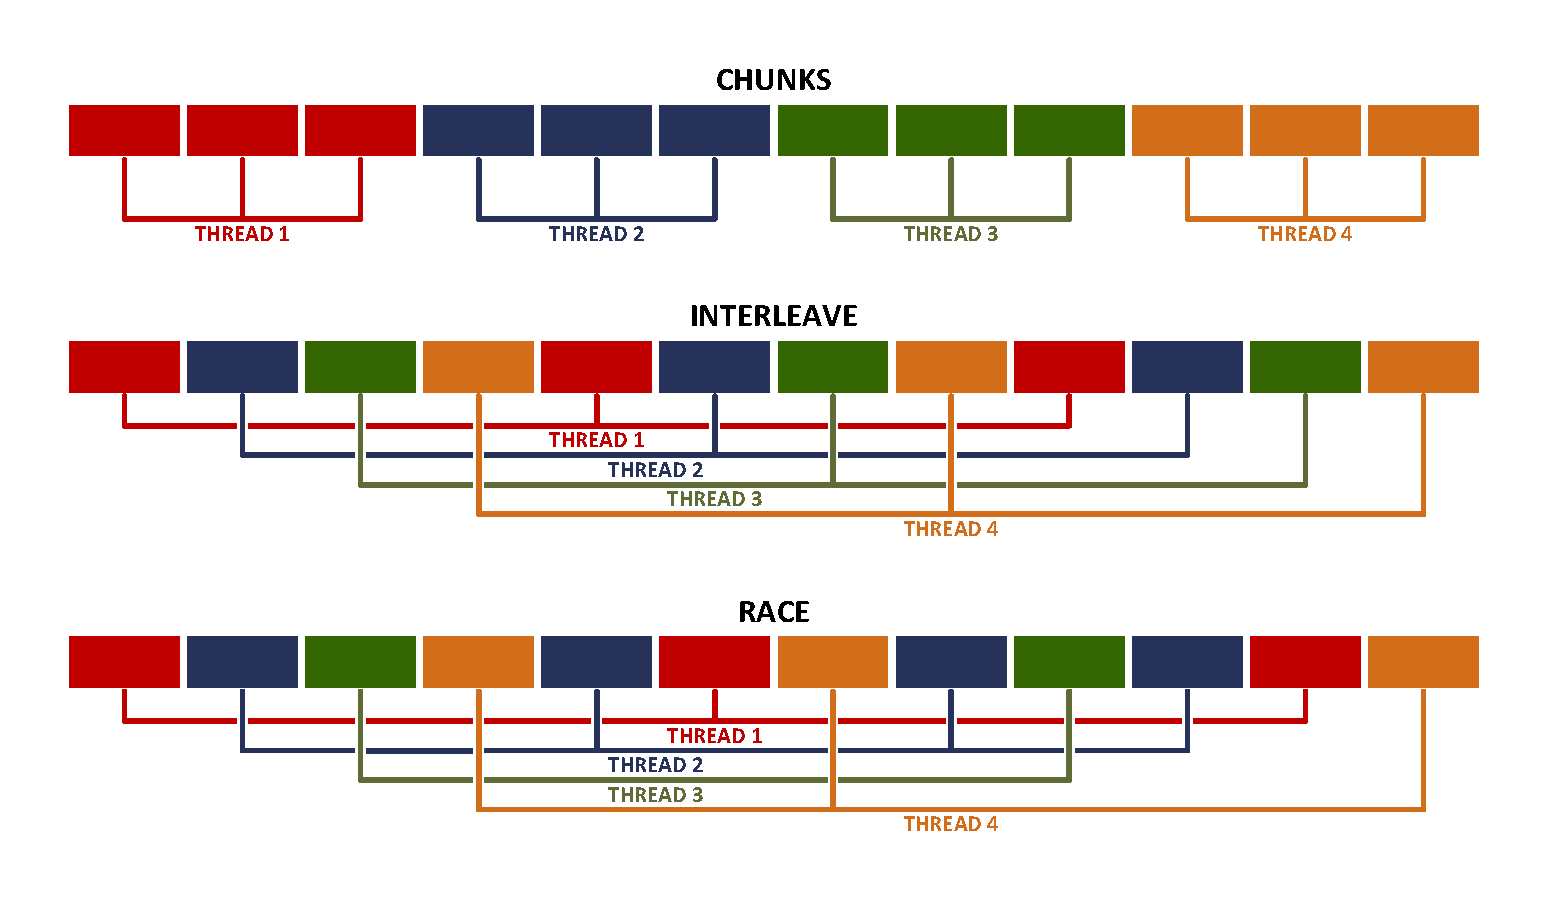
\includegraphics[width=0.8\textwidth]{./pics/text_3_omp1/modes.pdf}
\singlespacing
\captionstyle{center}\caption{Иллюстрация работы трех рассматриваемых стратегий распараллеливания вычислений: CHUNKS\label{term:parallel_strategy_chunks}, INTERLEAVE\label{term:parallel_strategy_interleave}, RACE\label{term:parallel_strategy_race}.}
\label{fig:text_3_omp1_modes}
\end{figure}

В качестве первой стратегии распараллеливания была использована стратегия CHUNKS, в которой массивы входных данных были разделены на равные непрерывные части по числу используемых потоков, каждый поток обрабатывал свои участки массивов входных данных (на листинге~\ref{lst:text_3_strat_chunks} \texttt{nt} -- общее количество потоков, \texttt{solver\_16} -- указатель на решатель для обработки 16 экземпляров задачи Римана).

\begin{singlespace}
\begin{lstlisting}[caption={Распараллеливание римановского решателя с помощью стратегии CHUNKS.},label={lst:text_3_strat_chunks}]
#pragma omp parallel
{
    int tn = omp_get_thread_num();
    int lb = (int)((c/FP16_VECTOR_SIZE)*((double)tn/(double)nt));
    int ub = (int)((c/FP16_VECTOR_SIZE)*((double)(tn + 1)/(double)nt));

    for (int i = lb * FP16_VECTOR_SIZE;
         i < ub * FP16_VECTOR_SIZE;
         i += FP16_VECTOR_SIZE)
    {
        solver_16(dl + i, ul + i, vl + i, wl + i, pl + i,
                  dr + i, ur + i, vr + i, wr + i, pr + i,
                  d + i, u + i, v + i, w + i, p + i);
    }
}
\end{lstlisting}
\end{singlespace}

Во второй стратегии -- INTERLEAVE -- массивы входных данных были разделены на участки по 16 элементов и распределялись между потоками в шахматном порядке (на листинге~\ref{lst:text_3_strat_interleave} \texttt{c\_base} -- длина массивов входных данных без учета эпилога цикла, \texttt{nt} и \texttt{solver\_16} имеют тот же смысл, что и на листинге~\ref{lst:text_3_strat_chunks}).

\begin{singlespace}
\begin{lstlisting}[caption={Распараллеливание римановского решателя с помощью стратегии INTERLEAVE.},label={lst:text_3_strat_interleave}]
#pragma omp parallel
{
    int tn = omp_get_thread_num();

    for (int i = tn * FP16_VECTOR_SIZE;
         i < c_base;
         i += nt * FP16_VECTOR_SIZE)
    {
        solver_16(dl + i, ul + i, vl + i, wl + i, pl + i,
                  dr + i, ur + i, vr + i, wr + i, pr + i,
                  d + i, u + i, v + i, w + i, p + i);
    }
}
\end{lstlisting}
\end{singlespace}

Третья стратегия -- RACE -- основана на ведении глобального адреса следующего готового к обработке участка входных данных.
Как только очередной поток освобождается, он приступает к обработке следующих свободных 16 экземпляров задачи.
Таким образом, была предпринята попытка избавиться от простоев потоков в случае разного времени выполнения отдельных экземпляров задачи.
На листинге~\ref{lst:text_3_strat_race} \texttt{g} -- глобальный счетчик следующей свободной партии экземпляров задачи Римана, доступный всем потокам.
Для его проверки и продвижения требуется блокировка.

Для всех описанных стратегий были выполнены тестовые расчеты на одном узле суперкомпьютера МВС-10П.
Были выполнены запуски векторизованного решателя для различного количества потоков, начиная от 1 и заканчивая 288.
По результатам прогона собиралось время выполнения векторизованной версии точного римановского решателя для разного количества потоков.
Отдельно выполнялись прогоны для стратегий распараллеливания CHUNKS, INTERELEAVE и RACE.
По результатам прогонов были построены графики ускорения векторизованного распараллеленного римановского решателя, а также эффективности распараллеливания для всех трех стратегий, эти графики представлены на рис.~\ref{fig:text_3_omp1_main_graph}.

\begin{singlespace}
\begin{lstlisting}[caption={Распараллеливание римановского решателя с помощью стратегии RACE.},label={lst:text_3_strat_race}]
int g = 0;
#pragma omp parallel
{
    int i = 0;
    bool is_break = false;

    while (true)
    {
        #pragma omp critical
        {
            if (g >= c_base)
            {
                is_break = true;
            }
            else
            {
                i = g;
                g += FP16_VECTOR_SIZE;
            }
        }

        if (is_break)
        {
            break;
        }

        solver_16(dl + i, ul + i, vl + i, wl + i, pl + i,
                  dr + i, ur + i, vr + i, wr + i, pr + i,
                  d + i, u + i, v + i, w + i, p + i);
    }
} 
\end{lstlisting}
\end{singlespace}

\begin{figure}[ht]
\centering
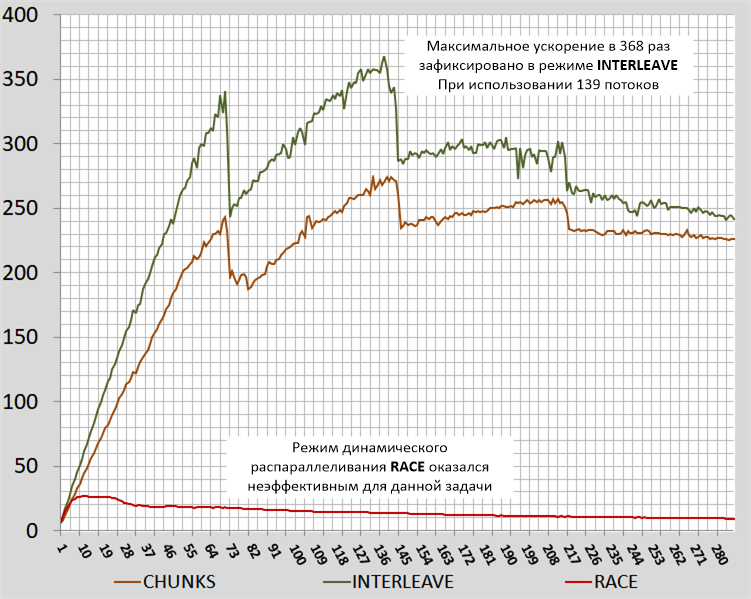
\includegraphics[width=1.0\textwidth]{./pics/text_3_omp1/main_graph.png}
\singlespacing
\captionstyle{center}\caption{График ускорения и эффективности распараллеливания векторизованного римановского решателя на микропроцессоре Intel Xeon Phi KNL.}
\label{fig:text_3_omp1_main_graph}
\end{figure}

Из рис.~\ref{fig:text_3_omp1_main_graph} видно, что стратегия распараллеливания RACE является нежизнеспособной даже на сравнительно небольшом числе потоков.
Блокировка глобального ресурса (счетчик следующей свободной партии задач), оказывается фатальной и приводит к простою потоков.

Из двух других стратегий стратегия INTERLEAVE показала себя лучше, продемонстрировав максимальное ускорение более 50 раз на 139 потоках.

На графиках явно просматриваются 4 характерные участка, длина которых совпадает с количеством ядер микропроцессора Intel Xeon Phi KNL 7290 (72 ядра).
На первом участке масштабируемость распараллеливания близка к линейной.
На втором участке наблюдается сначала некоторое снижение эффективности, но затем при дальнейшем увеличении количества потоков удается добиться дополнительного ускорения.
На третьем и четвертом участках графиков наблюдается снижение производительности.
Это ожидаемо, так как каждое ядро микропроцессора содержит два векторных исполнительных устройства и при запуске на ядре трех или четырех потоков с обработкой плотного векторного кода начинается конкуренция за эти исполнительные устройства.

Таким образом, можно сделать вывод, что оптимальным с точки зрения использования ресурсов микропроцессора Intel Xeon Phi KNL режимом распараллеливания вычислений на общей памаяти является использование стратегии INTERLEAVE (что соответствует использованию директивы \texttt{schedule} с параметрами \texttt{kind = static} и небольшом значении параметра \texttt{chunk}) c задействованием двух потоков на ядро.

%---------------------------------------------------------------------

После выбора стратегии распараллеливания плотного векторного кода на общей памяти на микропроцессоре Intel Xeon Phi KNL\label{abbr:knl4}, для этой стратегии проводились тестовые запуски на всех типах вычислительных узлов суперкомпьютера МВС-10П: Haswell, Broadwell, KNL, Skylake, Cascade Lake (характеристики узлов приведены в таблице~\ref{tbl:text_2_scaling_supercomputers}).
Для запуска использовались те же расчетны коды точного римановского решателя (скалярная и векторизованная версии).

На рис.~\ref{fig:text_3_omp2} сверху слева представлены графики ускорения скалярной версии римановского решателя при увеличении количества потоков с 1 до 160.
Для каждого вычислительного узла явно просматриваются отрезки квазилинейного ускорения, которые завершаются заметными провалами.
Длина этих отрезков во всех случаях равняется суммарному количеству ядер в узле, а провалы обусловлены конфликтами за аппаратные ресурсы.
При этом стоит отметить, что хоть максимальное количество доступных потоков для вычислительного узла на базе микропроцессора KNL равняется 288, однако на графике не показаны значения больше 160, так как сверх этого значения наблюдается только деградация производительности, и наиболее эффективное использование зафиксировано в районе 140 потоков.
Также можно отметить, что для всех микропроцессоров ускорение близко к линейному до тех пор, пока каждый поток запущен на своем отдельном ядре.

\begin{figure}[ht]
\centering
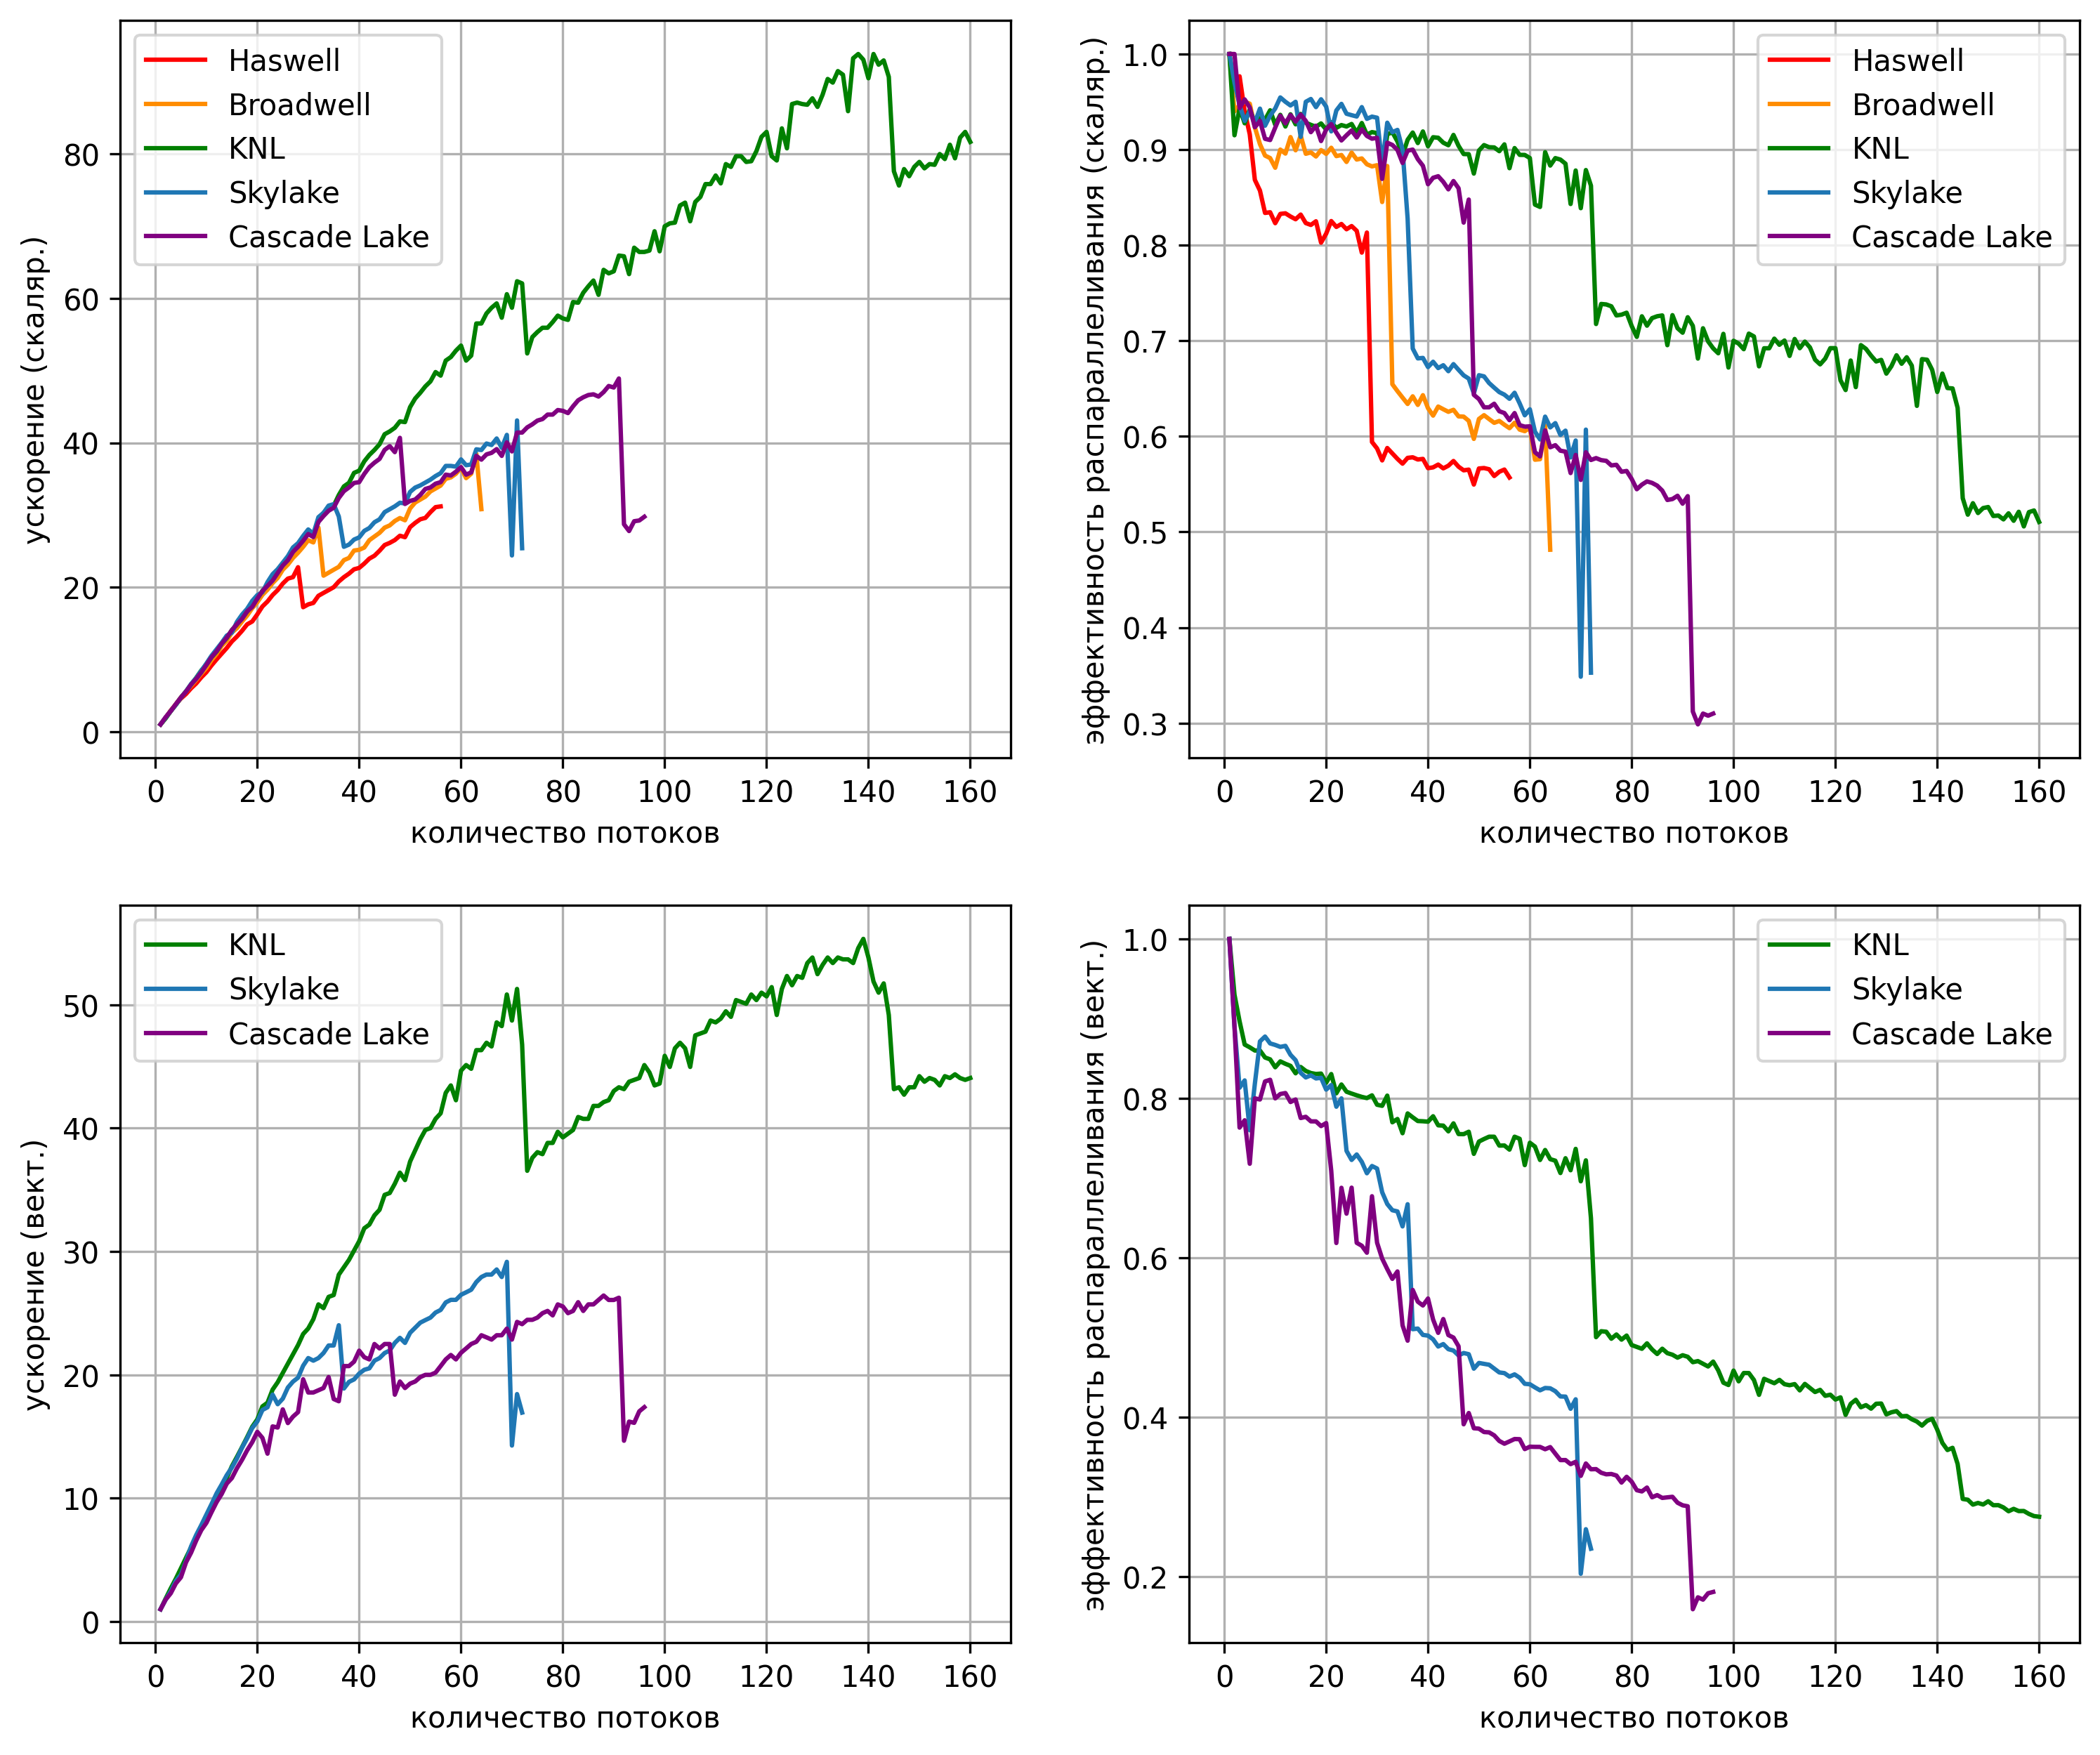
\includegraphics[width=1.0\textwidth]{./pics/text_3_omp2/main_chart.png}
\singlespacing
\captionstyle{center}\caption{Графики ускорения и эффективности распараллеливания скалярной и векторизованной версии римановского решателя для микропроцессоров Haswell, Broadwell, KNL, Skylake и Cascade Lake.}
\label{fig:text_3_omp2}
\end{figure}

На рис.~\ref{fig:text_3_omp2} снизу слева представлены аналогичные данные, но уже для векторизованной версии римановского решателя (соответственно только для микропроцессоров KNL, Skylake, Cascade Lake).
Из графиков видно, что характер ускорения для KNL практически не поменялся, тогда как Skylake и Cascade Lake демонстрируют серьезную деградацию ускорения вычислений уже на небольшом количестве потоков.

На рис.~\ref{fig:text_3_omp2} справа приведены данные показателей эффективности масштабирования римановского решателя (скалярной и векторизованной версии).
Эти иллюстрации более информативные.
Например, из рис.~\ref{fig:text_3_omp2} сверху справа видно, что эффективность распараллеливания при количестве потоков, не превышающем количество ядер вычислительного узла, находится для всех микропроцессоров на хорошем уровне в диапазоне 0,8-1,0.
Рис.~\ref{fig:text_3_omp2} снизу справа наглядно демонстрирует хорошую эффективность распараллеливания векторизованного римановского решателя для микропроцессора KNL с показателем, близким к 0,8 вплоть до использования 72 потоков, тогда как узлы на базе микропроцессоров Skylake и Cascade Lake деградируют на масштабировании векторизованной версии римановского решателя на достаточно небольшом количестве потоков.
